\begin{figure}
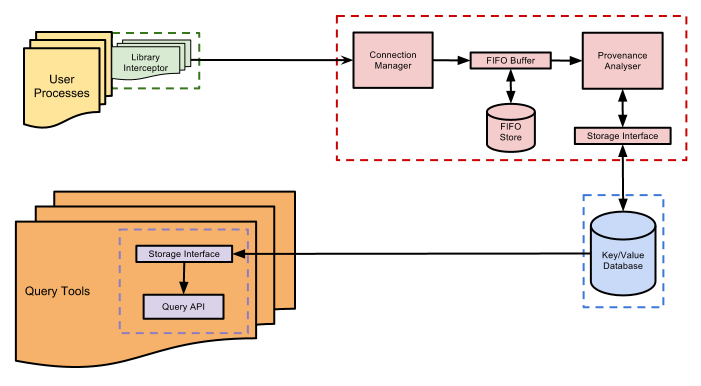
\includegraphics[width=\textwidth]{res/ProvDesign.png}
\label{fig:detdes}
\caption{Detailed design of the provenance system.}
\end{figure}

\subsubsection{Library Interceptor}
The front end will consist of a shared library implemented in C, which will be pre-loaded before the user application starts execution. The shared library can be loaded during the start of a shell session and will track all activities that the user performs during that session. The front end will monitor a subset of system calls and transmit raw system call data to the back end via a Unix domain socket. The data will be transmitted by using a specific protocol as described in Section \ref{ProvProt}. The front end will be implemented using a library called Purelibc, our justification of this choice can be found in Section \ref{PureLCJust}.

\subsubsection{Connection Manager}
The connection manager is a multi-threaded Unix domain sockets server which can accept connections from multiple front end instances and feed the raw system call information into a FIFO buffer module.

\subsubsection{FIFO Buffer \& FIFO Store}
The FIFO buffer module provides a dynamic and persistent FIFO storage to ensure that in an event when the provenance analyser is unavailable, the system will not lose current raw provenance information. The FIFO module also provides slack to compensate for variations in the system utilisation.

\subsubsection{Provenance Analyser}
The provenance analyser converts raw provenance data into logical provenance objects and relations. This is achieved by tracking active process IDs and the file descriptors that they possess. By maintaining this state and tracking new raw provenance data the system can trace new provenance entities being created and relations being formed. The system can then persist this information using the storage interface.

\subsubsection{Storage Interface}
The storage interface uses a key/value database to store provenance objects. It will present a strict interface to the rest of the system allowing provenance objects to be stored and retrieved and for iteration over ranges of provenance objects. We will be implementing this using an embedded key/value database called levelDB, our justification for such can be found in Section \ref{levelDBJust}. 

\subsubsection{Key/Value Database}
The key/value store will feature three levelDB databases, one acting as the main data store and two acting as indexes to this. The main database will map provenance identifiers (provID) to provenance objects (see section \ref{POF}). Provenance identifiers will be unique monotonically increasing integer identifiers, they will monotonically increase to allow for a strong mapping between time and provenance identifier. The first index will map entity names to a list of all provenance entities that hold that name, ordered by increasing provID. This will allow new entries to simply be appended to the list. The second index will map timestamps to appropriate provIDs, this will be filled by inserting entries at boundaries in timestamp(e.g. every hour or every minute) containing the timestamp and the last used provID. Thus by rounding a time period to the nearest boundaries you can obtain a range of provIDs that describes the time period.

\subsubsection{Query API}
The query API will provide a wide variety of functions for retrieving provenance objects from the storage interface. It will be available initially as an importable module which any query tool can use. The strict definition of it's API has not yet been created as further investigation into the form of provenance queries needs to be made.
